\section{BeeSAFE}

\begin{frame}
	\frametitle{BeeSAFE}
	
	\Large
	Developing a system able to autonomously coordinate a team of robots when exploring an
	environment. The project has involved two main activities:
	
	\vspace{0.4cm}
	
	\begin{itemize}
		\item \textbf{Multi-Robot SLAM}
		\item \textbf{Multi-Robot Task Allocation}
	\end{itemize}
\end{frame}

\begin{frame}
	\frametitle{BeeSAFE}
	
	\begin{center}
		\begin{tikzpicture}
			\node at (0,0) [draw=white,ultra thick,inner sep=0pt]
			{
				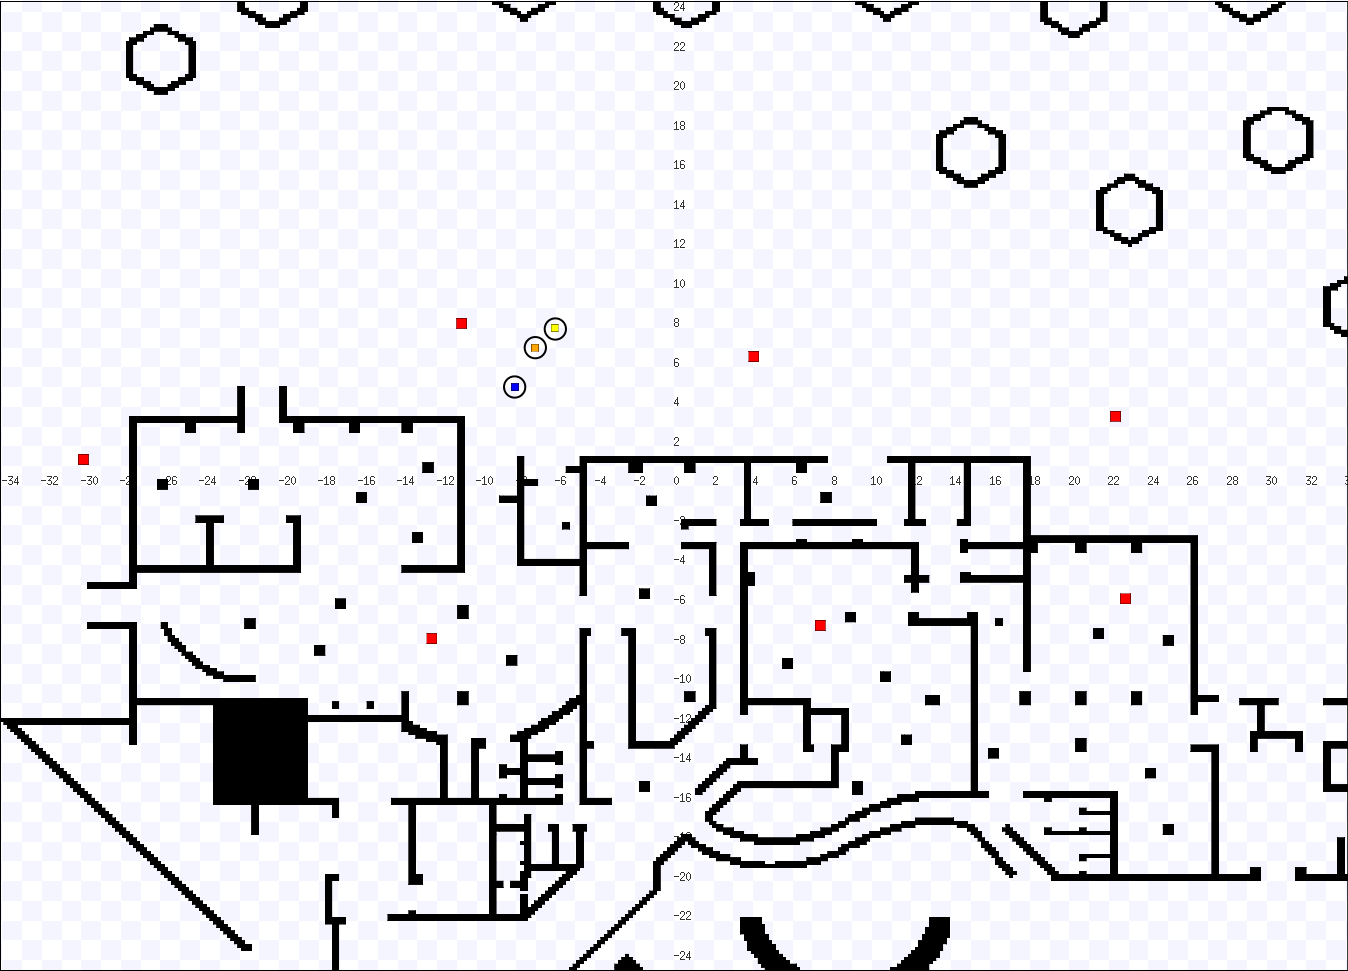
\includegraphics[scale=0.2]{Figures/BeeSAFE-Map}
			};
		\end{tikzpicture}
	\end{center}
\end{frame}

\begin{frame}
	\frametitle{BeeSAFE}
	\framesubtitle{Reconstructed map}
	
	\begin{center}
		\begin{tikzpicture}
			\node at (0,0) [draw=white,ultra thick,inner sep=0pt]
			{
				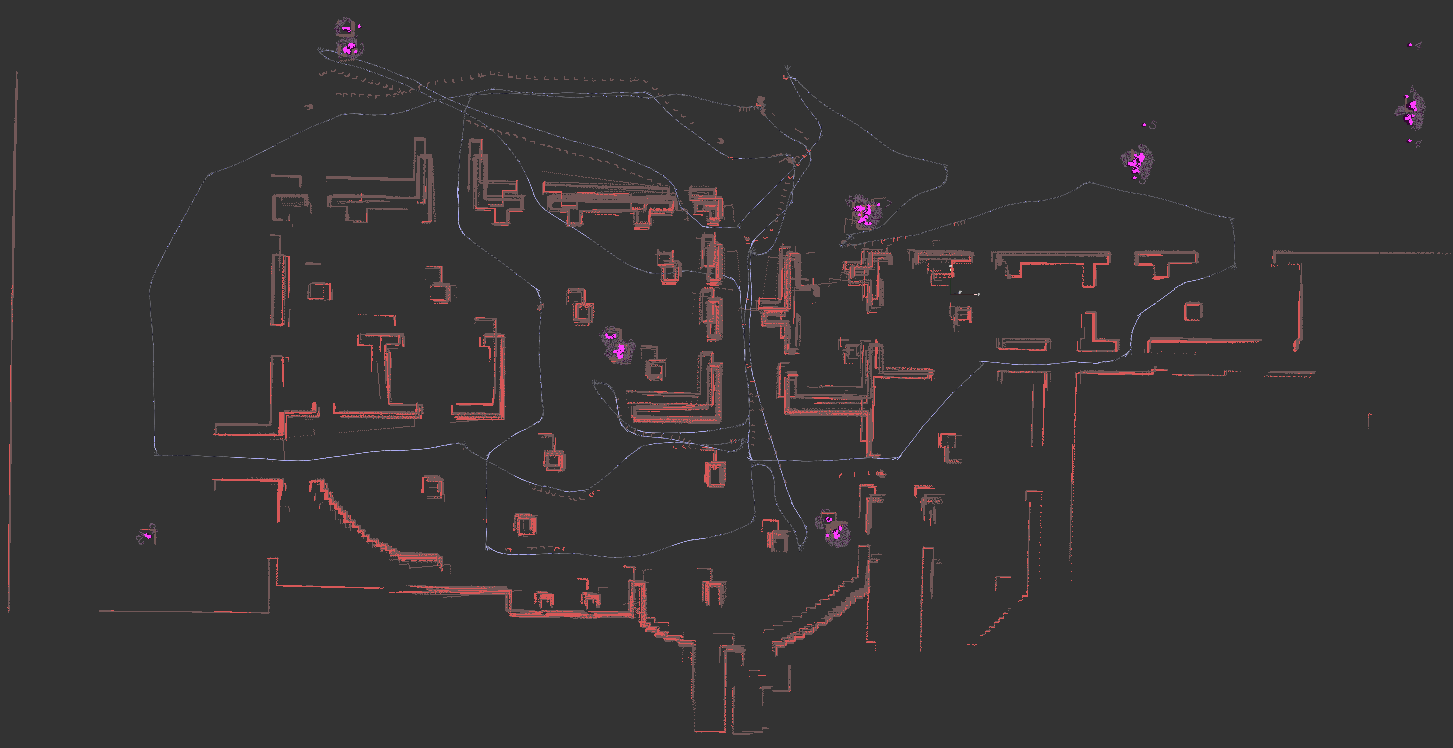
\includegraphics[scale=0.3]{Figures/BeeSAFE-ReconstructedMap}
			};
		\end{tikzpicture}
	\end{center}
\end{frame}

